\chapter{Approaching Word2Vec and ESN Language Model}\label{approach}

In this chapter we propose a model used to validate our hypothesis of using distributed embedding for improvement on thematic role assignment over grammatical construction with localist representation (see section for more details).

\section{Proposed Model}

To validate our hypothesis, we propose a Word2Vec-ESN language model for thematic role assignment task (see fig). The model is inpired from the one used by [ref] for thematic role assignment task[ref]. Word2Vec-ESN model is basically the combination of Word2Vec model and ESN (see fig). The word2vec model is used to generate distibuted embeddings of the words in input sentences. The generated embeddings are then input to ESN, which further processes these embeddings to learn and predict the thematic roles for the input sentence. 

\begin{figure}[hbtp]
\centering
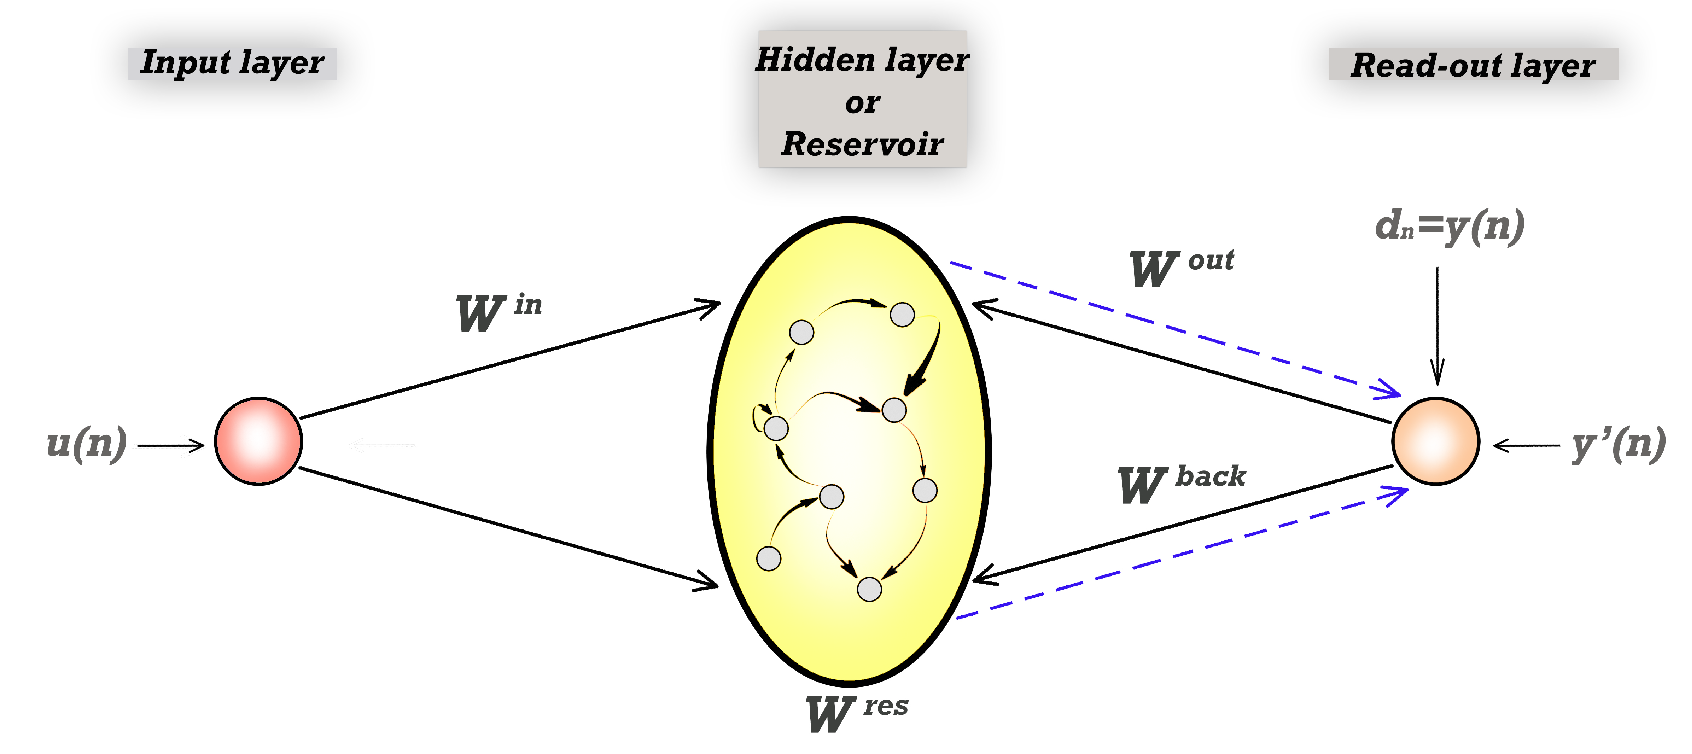
\includegraphics[width=0.8\linewidth]{esn_architecture}
\caption{\textbf{Architecture of classical ESN:} The reservoir is the recurrent neural network with N units and initialized with random connection. The reservoir is provided input from the input u(n) and y(n) from the input and output neurons  respectively. The input weights Win from input and Wback from output neurons are also randomly initialized and stays static during learning. The output  weight from reservoir to output unit is learned by the network.[ESN9]}
\label{fig:esn_arch}
\end{figure}

The Word2Vec model was trained using skip-gram negative sampling approach on a general purpose dataset (e.g. Wikipedia) and the domain specific dataset to learn the distributed embeddings for each word in the vocabulary(see section next). The reservoir of ESN, composed of leaky integrator neurons and sigmoids activations fuctions was randomly initilizied. A fixed fan-out of 10 and 2 is chosen for hidden-to-hidden and input-to-hidden connections respectively. In other words, each reservoir neuron is connected to 10 other reservoir neurons and each input neuron is connected to only 2 reservoir neurons. The input-to-hidden and hidden-to-hidden weights were generated sparse and randomly from a Gaussian distribution with mean 0 and variance 1. These weights once initialized are fixed and remains unchanged during training. The reservoir internal states for a given input sequence was accumulated across time which is then linearly combined with the desired output (thematic roles) using ridge regression to learn reservoir to readout weights. The reservoir internal states are simply the non-linear high dimensional expansion of input sequence[ref?]. Reservoir to readout weights are the only weights learned during training. The mathematical expressions for reservoir state updates and learning output weights are discussed in more details in section [ref]. The ridge regression was used rather than classical linear regression so as to avoid over-fitting and improve generalization capabilities, as it restricts the magnitude of readout weights[ref]. The learned readout weights can then later be used for generating coded meaning for the test sentences which were previously not seen by the model.

To ensure the objectivity of our findings we used two variants of the proposed models which were used to perform the experiments. Although both the variants are architecturally similar but varies in training objective and the evaluation metrics used evaluate the model performance. The number of units in input and output layer differs for each variation. Thus the input and output coding for ESN also differs depending on the training objective. The difference in variants is discussed in more details in next two subsection sections.

\subsection{Model Variant-1}

This variant of the model (see fig. \ref{fig:model_variant_1}) treats the thematic role assignment task as a prectition problem. The objective of the model variant is to predict the role of semantic words in a sentence with respect to a verb. To evaluate the performance of this model variant meaning error and sentence error metrics were used.(see section- Evaluation Metrics).

\begin{figure}[hbtp]
\centering
\includegraphics[width=0.8\linewidth]{model_variant_1}
\caption{\textbf{Word2Vec-ESN Model Variant-1:} The figure shows the processing of a sentence by the model variant at time step 1. Nouns and verbs (specified in orange and green respectively) are stored in a memory stack for interpretating coded meaning. The word 'John' is input to word2vec model which generate a word vector of $E_{v}$ dimensions. The output vector is then input to ESN for further processing. During training the readout units are presented with the coded meaning of the input sentence(i.e. N1-A1: Noun-1 is Agent of verb 1, N2-O1: Noun-2 is object of verb 2). In testing, the readout units codes the predicted meaning of input sentence. The meaning: hit(John,ball,--) is decoded by mapping the thematic roles predicted by readout neurons with nouns and verbs from memory stack. Adapted from \cite{xavier:2013:RT}} 
\label{fig:model_variant_1}
\end{figure}

The training sentences are presented to the model one at time, word-by-word across time. We initially prepare two memory stacks, one for storing nouns and one for storing verbs (see fig \ref{fig:model_variant_1}). Word2Vec model then receives the input word and generate the vector embedding of $E_{v}$ dimensions which is then input to the ESN. The input layer of ESN uses these distributed embeddings as input features for learning and predicting thematic roles of the sentences. Thus the size of input layer is same as the dimensionality of word vector i.e. $E_{v}$. The output of reservoir is accumulated for each time step during the presentation of a sentence. The reservoir states are reset before the presentation of the consequent sentence. The size of readout layer depends on the maximum number of semantic words (e.g. nouns and verbs) a sentence can have in the corpus. A noun can have one of the three possible roles: Agent, Object and Recipient, with respect to a verb. For example, if the sentences in the corpus have maximum of $N_{n}$ nouns and $N_{v}$ verbs then the readout size would be $N_{n} \times N_{v} \times {3}$  neurons; each output neuron encodes the thematic role of a semantic word (e.g. noun). The output neurons have an activation of 1 if corresponding thematic role is present for the sentence, -1 otherwise. The accumulated reservoir states are then linearly combined with readout activations to learn the reservoir-to-readout weights.

This model variant can be operated in two learning modes, so that it learns to extract the coded meaning of each noun with respect to a verb.

\begin{enumerate}
\setlength{\itemsep}{\smallskipamount}

\item \textbf{Sentence Continuous Learning Mode}: In this learning mode learning takes place from the beginning of the sentence till the end of sentence or in other words the teacher labels (coded meaning) for the sentece is made availabel to model from the onset of first word in sentence. Thus, the regression is applied with teacher labels from the onset of first word in the sentence. \label{eg:SCL}

\item \textbf{Sentence Final Learning Mode}: In this mode the learning takes places only at the end of the sentence. Hence, the teacher labels are only provided to the network at the end of sentence i.e. from last word of the sentence to the final period. \label{eg:SFL}

\end{enumerate} 

\subsubsection{Decoding Output}

As described earlier, coded meaning of sentence is defined as the description of thematic roles for all the semantic words (e.g. nouns,verbs etc.) in the sentence (see fig). As the readout neurons codes the thematic roles for individual semantic words, word level coded meaning were obtained in two steps. For every semantic word (e.g. noun) the readout activity is threshold at 0 and then the maximum of all the activations between 3 possible roles (i.e. Agent, Object, Recipient) is taken as the coded meaning of this semantic word. A semantic word is said to have incorrect coded meaning if the winning readout neurons is not the correct role of the semantic word. If there is no activation above threshold for a semantic word, then this semantic word is considered to have no coded meaning. The coded meaning of the sentence can then be interpreted from the the word level meaning by mapping the nouns and verbs from the memory stack created before giving the sentence to the model (see fig \ref{fig:model_variant_1}).

\subsubsection{Evaluation Metrics}

To evaluate the performance of this model variant two error measures were evaluated: the meaning error and the sentence error. Meaning error is the percentage of semantic words with incorrect coded meaning, whereas the Sentence error is the percentage of sentences having at least one semantic word with incorrect coded meaning [ref. xavier paper]. Both the error measure are related but there is no strict corelation between them. Sentence error is a more stricter measure than meaning error to evaluate model performance because a meaning error of $5\%$ cannot be used to estimate the sentence error, as these $5\%$ incorrect words can be from just one sentence or several sentences. 

For the analysis not all the readout neurons are considered i.e. if a sentence have only 2 semantic words then only readout neurons corresponding to these two semantic words were analyzed [ref.]. If there are more than one verb, in a sentence then each semantic word can have possible role with respect to each verb. Thus readout neurons corresponding to the mapping of semantic word and the verbs are used for analysis. For example in the sentence "John threw the ball and then he caught it". Each semantic word "John" and "ball" can have possible roles with verbs "threw" and "caught". So there are 4 possible output mappings for both the semantic words to their coded meaning. 

\subsection{Model Variant-2}

This variant of the model process the sentence differently from variant-1 and consider thematic role assignment task as a classification problem. The training objective is classify the words in the sentences to one of the roles namely Verb, Agent, Object, Recipient and XX (No-role) and maximize the the classification scores (i.e. F1-score, Precision and Recall- see section-) for each role. 

Training sentences are presented to the model sequentially, word by word. Two input features plays an important role in this model variant: argument and predicate, with argument describing the current word being processed and predicate describes the verb with respect to which argument is processed. So, if there are $N_{v}$ verbs in a sentence than the sentence is processed $N_{v}$ times. Each argument then takes a unique role for an argument-predicate pair. For example in the following sentence there are two predicates namely 'chased' and 'ate'. Thus this sentence will be processed twice and each argument will take a role for an argument-predicate pair.

\begin{table}[!htb]
\centering
\label{tab:argument-predicate}
\begin{tabular}{lccccccccc}
Arguments           & the & dog & that & chased & the & cat & ate & the & rat \\
Predicate('chased') & XX  & A   & XX   & V      & XX  & O   & XX  & XX  & XX  \\
Predicate('ate')    & XX  & A   & XX   & XX     & XX  & XX  & V   & XX  & O  
\end{tabular}
\end{table}

 At any time instant an argument and the predicate is input to the model where initially Word2vec model generates the distributed embeddings for both the input words. The generated word embeddings are concatenated and then taken by ESN as an input. Thus the size of ESN input layer is $2 \times E_{v}$ where the first $E_{v}$ neurons takes the vector representation of the argument and remaining $E_{v}$ neurons for the predicate. The reservoir internal states are collected for an input sequence over time which will be used later for regression with the desired output. The readout layer have 5 neurons each coding for a role. An output neuron have an activation 1 if the input argument have the corresponding role, -1 otherwise. The regression is performed with collected reservoir states and the readout activations to learn the reservoir-to-readout weights. Figure\ref{fig:model_variant_2} shows the processing of an example sentence by the model variant.

\begin{figure}[hbtp]
\centering
\includegraphics[width=0.8\linewidth]{model_variant_2}
\caption{\textbf{Word2Vec-ESN Model Variant-2:} 
The figure shows the process of a sentence in model variant-2 at time step 1. At any instant of time an argument (current word, marked in orange) and predicate (verb,marked in green) is input to the model. Word2Vec model generates the word vectors of $E_{v}$ dimensions which are then cocatenated to form a $2 \times E_{v}$ dimensions(shown in orange and green color). ESN takes the resultant vector for further processing. During learning, the readout neurons are presented with the role of input word (i.e. A (Agent)). The read-out weights (shown in dashed line) are learned during training. During testing the readout unit codes the role of input words, which are then accumulated and decoded to meaning \textit{hit(John,ball,--)} at the end of sentence. Inspired from \cite{xavier:2013:RT}
}
\label{fig:model_variant_2}
\end{figure}

\subsubsection{Decoding Output}



\subsubsection{Evaluation Metrics}

To analyze the performance of this model variant, the confusion matrix or contigiency table (Kohavi and Provost, 1998) was build and classification scores were calculated for all possible roles: Accuracy, Precision, Recall and F1-Score. The classification scores were then averaged, weighted by support (number of true samples for each roles), to get a single real numbered scores. Weighting the average score by support takes into account the role imbalance in the dataset. The same evaluation metrics was used for CoNLL-04 and CoNLL-05 Semantic Role Labelling task[ref.].

%draw confusion matrix from actual data

The confusion matrix describes the prediction made by the model. The rows of the matrix corresponds to the actual roles available in the dataset and the columns corresponds the predictions made by the model. The diagonal elements of this matrix represent the number of words for which the predicted role is equal to the true role,  whereas all the non-diagonal elements represents the number of word which were labelled incorrectly. As the values of diagonal elements of confusion matrix indicates number of correct predictions so higher the values of diagonal elements the better.

Using the confusion matrix accuracy can be calculated as ratio of number of correctly labelled words to total number of words (equation \ref{eqn:accuracy}). This meaures specifies how often the classifier is correct. 

\begin{equation}\label{eqn:accuracy}
Accuracy= \frac{\text{number of words correctly labelled}}{\text{total number of words}}
\end{equation}
 
However this measure can be distorting when the  dataset have words with large role imbalance as it gives high scores to models which just predict the most frequent class and cannot be used alone to evaluate the model performance[ref.]. In our dataset we have imbalanced roles as most of words have labels "XX" (No Role) compared to other roles. Thus we needed additional measures such as Precision, Recall and F1-score to evaluate the model. All these scores are reported as a value between 0 and 1. 

Precision is defined as ratio of True positive (TP) to False Positive(FP) and True Positive (equation \ref{eqn:precision}). It is the measure of the accuracy of a role provided that a specific role has been predicted. 

\begin{equation}\label{eqn:precision}
Precision= \frac{\text{True Positive}}{\text{True Positive + False Positive}}
\end{equation}

In the confusion matrix above, the precision for the role Agent(A) would be calculated as:

\[Precision(A) = \frac{TP_{A}}{(TP_{A}+E_{BA}+E_{CA})}\]

Recall is defined as the ratio of True Positive to True Positive and False Negative. It measure how good a model is labelling the correct roles. It is also called Sensitivity or True Positive Rate.

\begin{equation}\label{eqn:precision}
Recall= \frac{\text{True Positive}}{\text{True Positive + False Negative}}
\end{equation}

Recall for the role Agent, in above confusion matrix will be:
\[Precision(A) = \frac{TP_{A}}{(TP_{A}+E_{BA}+E_{CA})}\]

F1-Score is the harmonic mean of precision and recall. In other words, it represents the balance between the precision and recall and is calculated as:

\begin{equation}\label{eqn:precision}
F1= 2\times \frac{\text{Precision} \times{Recall }}{\text{Precision + Recall}}
\end{equation}

\section{Comparision of Model Variants}




\section{Dataset and pre-processing}

\subsection{Corpus For TRA Task}

For the experiments we used corpus of 462 sentence and 90582 sentences. The same corpus was used in thematic role assignment in [ref?]. The sentence in corpus-462 was generated using a context-free-grammer for English language. Each sentence in this corpus can have verbs which can take 1, 2, or 3 arguments. For example sentences, “The man jump” , “He cut an Apple” , “John gives ball to Marie” have 1 , 2 and 3 arguments respectively)[ref]. The sentences in the corpus have a maximum of four nouns and two verbs. A maximum of 1 relative clause is present in the sentences; verb in the relative clause could take 1 or 2 arguments (i.e., without recipient). For e.g. “The dog that bit the cat chased the boy”. The coded meaning for each sentence is described in order of Predicate, Agent, Object and Recipient. 

	Corpus-90582 consist 90582 sentences along with the coded meaning of each sentence. This corpus is redundant; multiple sentences with different grammatical structure have the same coded meaning (see fig). In total there were only 2043 distinct coded meanings[ref] . This corpus also have an additional property that along with complete coded meanings for sentences it also have incomplete meanings. For e.g. the sentence “The Ball was given to the Man” have no Agent, and Thus the meaning of the sentence is give(-,ball,man) [ref]. The corpus also contains 5268 pair and 184 triplets of ambiguous sentences i.e., 10536 and 553 sentences respectively. Thus in total there were 12.24 \% (i.e., $ 5268 \times 2+184*3=11088 $) of ambiguous sentences which have the similar grammatical structure but different coded meaning. 
Both the corpus-462 and corpus-90582 have the constructions in form:

walk giraffe <o> AP </o> ; the giraffe walk -s . \# ['the', 'X', 'X', '-s', '.']
cut beaver fish , kiss fish girl <o> APO , APO </o> ; the beaver cut -s the fish that kiss -s the girl . \# ['the', 'X', 'X', '-s', 'the', 'X', 'that', 'X', '-s', 'the', 'X', '.']

Each construction in the corpus is divided into four parts. The first part describes the meaning of sentence using Semantic words(or Open class words) in order of Predicate, Agent, Object, Recipient. The second part describes the order of thematic roles as appears in the raw sentence. The third part is the raw sentence with verb inflections and the fourth part is the abstract grammatical construction of sentence with Semantic words removed.

	We preprocessed these constructions, to obtain the raw sentences without verb inflections. Firstly all the words are lower cased and then the verbs with inflection is modified and replaced by conjugated verb. The verb conjugation to be used depends on the inflections the verb has. For e.g “The giraffe walk -s” has been changed to “The giraffe walks”. The reason replacing verb and its inflections with verb conjugation is that we have distributed word representation which captures this syntactic relations e.g walks-walk=talks-talk. We also added additional token <start> at the beginning of sentence and <end> token at end to mark the beginning and end of a sentence.
  
\subsection{Corpus For Training Word2Vec Model}

To train the word2vec model, we used wikipedia corpus to obtain the word embedding of words.
% Give properties of dataset here
 We chose to use Wikipedia data because we need to have vector representation of words and more words you have the better the vector representation. The Word2Vec model do not give good vector representation for words when trained over a small corpus thus a general purpose data set with billions of words is required to have good word embeddings. Once the vector representation of Wikipedia data is obtained the model can be trained further on any our domain specific dataset (corpus-462 and corpus-90582) with more bias toward (by repetition of dataset during training) domain specific dataset to update the previously learned vector representations. 

\section{Word Embeddings}

To get the vector representation of words we first trained a word2vec model on Wikipedia dataset. For training we used Word2vec skip-gram negative sampling (see Chapter 2 for more details) approach to obtain the word embeddings as it is claimed to produce better representation as compared to CBOW approach and is faster to train[ref?]. We used the hidden layer of with 50 units (desired dimensions of word embedding), and  a context window of length +-5. The negative sampling size is chosen to be 5 i.e. 5 noise words are chosen randomly from the vocabulary which does not appear in the context of the current input word. We ignored all the words which appears less than 5 times in the corpus. For network weight update stochastic gradient, the initial learning rate was set to be $\alpha=0.025$, which drops to $min_alpha=0.0001$ linearly as training progresses. 

The word embeddings obtained from training on Wikipedia dataset are good enough to capture the semantic relationship for e.g. $vec(Paris)-vec(France)+vec(Germany)\approx vec(Berlin)$. But the limitation was that once the vocabulary is created from the wikipedia dataset, it was not possible add new words in the vocabulary. However there is a possibility that some of the domain specific corpus is used to train the model in extension to wikipedia corpus some words may not be present in vocabulary generated while training on wikipedia corpus. Thus we needed to update the vocabulary of the model if the word is not present in order to facilitate online training of Word2Vec model. Unfortunately neither C++ API[ref?] nor Gensim python API[ref?] implementation of Word2Vec supports vocabulary update if once created. So, adapting the idea suggested by [ref Radim and Dr, Rutu Mulkar-Mehta], we implemented the online training of word2vec by extending Gensim API. The new words not present in existing vocabulary is added and initialized with some random weights, which can then be trained in usual manner to have vector embeddings. Although now the vocabulary can be updated in online manner but the vector embedding of newly added word have poor quality if its count in new corpus is few. This can be improved by repetition of new dataset several times before training the model [ref? Google group gensim].

So now when we have an online version of training word2vec model, we extend word2vec model by resuming training on corpus-462 and corpus-90582. While updating the model on new dataset we do not disregard any words irrespective of the count, so that we have vector embeddings of all the words in our corpus. Once trained the vector embeddings are normalized using L-2 norm before using them for further use. 

